% !TEX root = 0_main.tex
\chapter{Preliminaries and Background}\label{chap:prelim}
In this chapter,
-we provide general background information about secure multi-party computation
-we also introduce the generalized problem of secure function evaluation (SFE). and it two-party version and the threat model.
-Then we explain the Yao's Garbled Circuit protocol that enables two-party SFE for honest-but-curios adversary.
-We also explain the theoretical advancement and optimization on the protocol.
-Then we explain basics about combinational and sequential Boolean circuits.

\section{Secure Multi-party Computation}
the general problem of secure multi-party computation:
We have mutually suspicious parties that each has a private attribute (e.g., salary) and wish to compute a joint function (e.g., ) on their attributes.
They have to use some distributed protocol to evaluate and learn the output of the function without leaking their private information to other parties.
If we could find a third party that all the individuals trust, they could give her the inputs and she computes the function and returns the result to the parties.
Of course such a trusted party cannot be found in real scenarios of distributed systems.
Thus at best, we can emulate such a trusted third party with a cryptographic protocol~\cite{goldreich2013general}.
\fig{fig:multi-party-model} shows the idea model with a trusted third party and its emulation in a real model using a secure multi-party computation protocol.

\begin{figure}[ht]
    \centering
    \begin{subfigure}[tl]{0.35\textwidth}
        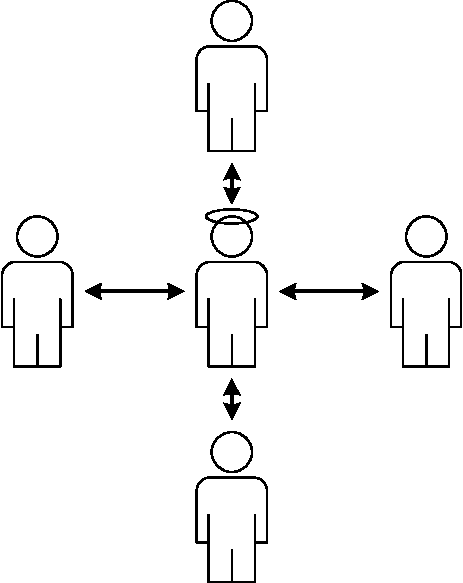
\includegraphics[width=\textwidth]{emulate_ideal-crop.pdf}
        \caption{Ideal Model}\label{fig:ideal-model}
    \end{subfigure}
		~~~~
    \begin{subfigure}[tr]{0.35\textwidth}
        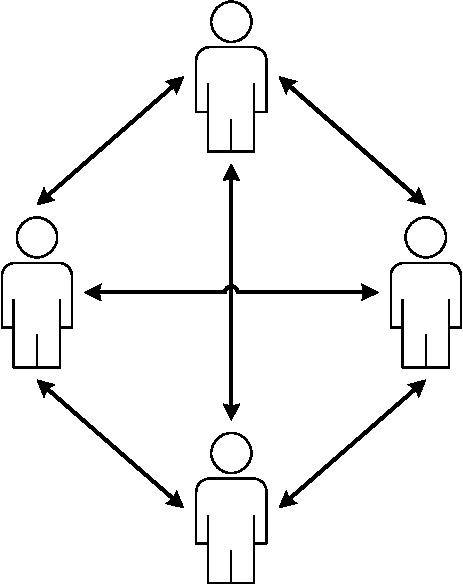
\includegraphics[width=\textwidth]{emulate_real-crop.pdf}
        \caption{Real Model}\label{fig:real-model}
    \end{subfigure}\\
    \caption{Emulation of a trusted third-party in secure multi-party computation (schematic based on~\cite{goldreich2013general}).}\label{fig:multi-party-model}
\end{figure}

Such emulation is possible under assumption about the emulation such as security level and type of the function that can be evaluated.
Initial general protocols Yao's Garbled Circuit Protocol GMW that are able to evaluate general functions.
Homomorphic encryption and Shamir's secret sharing are able to evaluate special function such as addition and multiplication.
In this thesis, we focus on the general secure multi-party computation where arbitrary desired function can be evaluated by the protocol.

\section{Secure Function Evaluation Definition}
The general secure multi-party computation is also known as secure function evaluation (SFE). It can be defined as follow: p parties each have an attribute: i1, ... ip. They want to compute function o = f(i1,i2, .. ip) where o is a tuple (o1, o2, ..., op) such that ok belongs to the kth party.
the function f can also be described as a tuple of functions f = (f1, f2, ...,  fp) where the output of fk(p1, p2, .. pm) = ok belongs to kth party.
(A common special case is that fi's are the same and all parties revives the same output. For example in case of the average of salaries, the result of the average function is evaluated and shared with all the participating parties).

\section{Two-Party Secure Function Evaluation}
two-party SFE is an important special case of general secure multi-party computation that was solved initially by Andrew Yao and GMW.
There are two parties Alice and Bob each has an input a and b and they want to compute (o1, o2) = (f1(a,b), f2(a,b)) where o1 belong to Alice and o2 belongs to Bob.

\begin{figure}[ht]
\centering
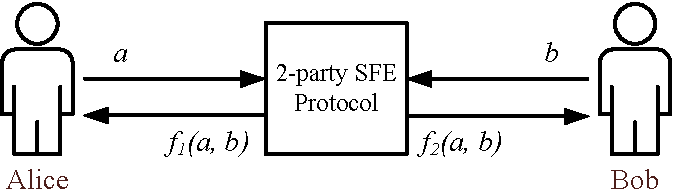
\includegraphics[width=0.70\textwidth]{two_party_SFE-crop.pdf}
\caption{The two-party secure function evaluation (SFE) protocol.}
\label{fig:globalflow}
\end{figure}

\section{Adversary Model}
We assume that all the parties are semi-honest which means that they follow the protocol exactly as specified without deviation or malicious behavior but they try to learn as much as possible about the other party's input from the information they receive during the protocol.
This model is often called honest-but-curious (HBC) adversary model in the literature and it is the basis for building a stronger security protocol.

In related work chapter \ref{chap:related}, we mention some of the recent approaches to extend the adversary model for two-party SFE to make it secure against the malicious adversary who can deviate from the protocol.

\section{Oblivious Transfer}\label{sect:prelim-OT}
Oblivious Transfer (OT)~\cite{NaorP05} is a cryptographic protocol based on public key encryption executed between two parties: Alice (sender) Alice and Bob (receiver).
Through OT, Bob selects and receives one message from a pair of messages provided by Alice without revealing his selection to her.
More formally, in a $1$-out-of-$2$ OT protocol ($\textrm{OT}^2_1$), Alice holds a pair of messages $(m_{0},\, m_{1})$; Bob holds a selection bit $b \in {0,1}$ and obtains $m_{b}$ without revealing $b$ to Alice and learns nothing about $m_{1-b}$.

\section{Yao's Garbled Circuit Protocol}\label{sect:prelim_gc}
Yao's Garbled Circuit protocol~\cite{Yao86} allows two parties Alice, called the \textit{Garbler} and Bob, called the \textit{Evaluator}, to jointly compute a function $o = f(x, y)$ on their private inputs $x$, provided by Alice and $y$, provided by Bob such that none of them reveal their inputs to each other.
In the end, one or both of them learns the output $o$.
The steps of Yao's protocol are described below.

\begin{enumerate}[label=\roman*.]
\item The function $f$ to be computed is represented as a Boolean circuit, called \textit{netlist}, consisting of 2-input 1-output logic gates (a four entry truth table).
\item For each wire $a$ in the netlist, Alice assigns two $k$-bit random strings, called \textit{labels}, $X_a^{0}$ and $X_a^{1}$ respectively corresponding to 0 and 1 Boolean values.
      $k$ is the security parameter -- typically $k=128$ is sufficient~\cite{bellare2013efficient}.
\item For each gate, she encrypts the output label in each row of the truth table with the corresponding input labels.
      The resulting table of ciphertexts is then randomly rearranged and called the \textit{garbled table}.
\item She then sends the garbled tables along with the labels corresponding to her input values to Bob.
      Bob obtains the labels corresponding to his input values obliviously through 1-out-of-2 OT protocol.
\item Bob uses these input labels to decrypt the garbled tables gate by gate.
      The label for the output wire of one gate are the label(s) for the input wire(s) of the subsequent gate(s).
\item In the end, Bob learns the labels for the final output wire and Alice has its mapping to 0 and 1, so that the actual value of the output can be determined.
\end{enumerate}

\section{Recent Improvements on the GC Protocol}
Throughout the years, the GC protocol has gone through a number of optimizations that reduce its computation and communication.
We describe the most important optimizations here.

\subsection{Free XOR~\cite{kolesnikov2008improved}}
The most significant optimization to GC so far is \textbf{\textit{Free XOR}} proposed in~\cite{kolesnikov2008improved}.
In this optimization, for any wire $a$, Alice only generates the label $X_a^{0}$ and computes the label corresponding to 1 as $X_a^{0}\oplus (R \parallel 1)$ where $\parallel$ represents bit concatenation and
$R$ is a global random ($k-1$)-bit value known only to Alice.
With this convention, the label for the output of an XOR gate with inputs $a$, $b$ and output $c$ can simply be computed as $X_{c} = X_{a} \oplus X_{b}$.
Thus it does not need computation or transfer of the garbled tables and the XOR gate becomes \textit{free}.

\subsection{Row Reduction~\cite{naor1999privacy}}
This optimization reduces the size of the tables for the non-XOR gates by $25\%$.
Here, instead of generating a label for the output wire of a gate randomly, the output label is produced as a function of the labels of the inputs.
Alice generates the output label such that the first entry of the garbled table becomes all $0$ and no longer needs to be sent.

\subsection{Garbling With a Fixed-key Block Cipher~\cite{bellare2013efficient}}
This method allows to efficiently garble and evaluate non-XOR gates using fixed-key AES.
In this garbling scheme which is compatible with the Free XOR and Row Reduction techniques, the output key $X_{c}$ is encrypted with the input label $X_{a}$ and $X_{b}$ using the encryption function $E(X_a,X_b,T,X_c) = \pi(K) \oplus K \oplus X_c$, where $K=2X_a\oplus4X_b\oplus T$, $\pi$ is a fixed-key block cipher (e.g., instantiated with AES), and $T$ is a unique-per-gate number (e.g., gate identifier) called \emph{tweak}.
The proof of security is given in~\cite{bellare2013efficient}.

\subsection{Half Gate~\cite{zahur2015two}}
The \textbf{\textit{Half Gate}} method~\cite{zahur2015two} utilizes both free-XOR and row reduction and reduces the cost of AND gates by an additional $25\%$.

\section{Boolean Circuits}
In SFE, the parties are able to evaluate a function on their private inputs.
In a number of SFE protocols including Yao's Garbled Circuit and GMW, the function has to be represented as a Boolean circuit.
In this context, Boolean circuit can be defined as a directed graph where nodes are Boolean gates (e.g., AND, OR, NOT, XOR, etc.) and inputs and edges are wires connecting the gates.

\subsection{Combinational Boolean Circuits}
The conventional Boolean circuits that are used in Yao's seminal work and later works on GC and GMW are combinational Boolean circuit.
Combinational circuit is a circuit whose graph does not have a loop and all the paths start from the inputs to outputs.
The combinational circuit can be modeled as a directed acyclic graph.

Yao's GC algorithm allows secure evaluation of a Boolean circuit, i.e., an acyclic graph of binary gates (e.g., AND, OR, XOR, etc.).
In digital circuit theory, such a circuit is called \emph{combinational circuit} and defined as a memory-less circuit in which outputs are functions only of inputs, see \fig{fig:combinational}.

\begin{figure}[ht]
    \centering
    \begin{subfigure}[t]{0.35\textwidth}
        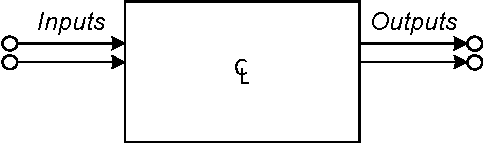
\includegraphics[width=\textwidth]{combinational-crop.pdf}
        \caption{Combinational circuit}\label{fig:combinational}
    \end{subfigure}
    \begin{subfigure}[t]{0.30\textwidth}
        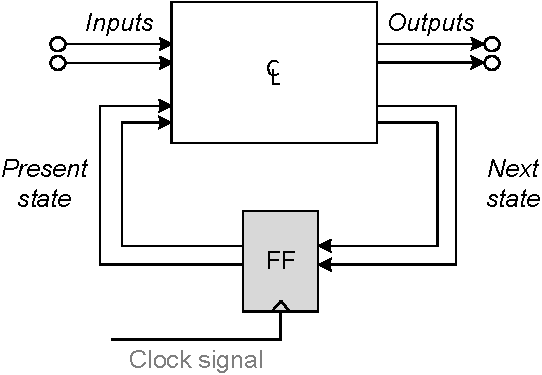
\includegraphics[width=\textwidth]{sequential-crop.pdf}
        \caption{Sequential circuit}\label{fig:sequential}
    \end{subfigure}\\
    \caption{(a) Combinational circuit where outputs are functions of only inputs. (CL represents Combinational Logic.)
    (b) Sequential circuit where outputs are functions of inputs and present states.
    }
\end{figure}

\subsection{Sequential Boolean Circuits}
In digital circuits, sequential circuit is a type of circuit that its output depends on the input and the state of the circuit stored in its memory elements.
Sequential circuit is similar to combination circuit except for the new memory elements called flip-flops.
A flip-flop stores the value of its input wire (usually denoted by D) to be reused later (denoted by Q) as the circuit state.
A periodic square signal called clock are used to synchronized sampling the value in flip-flops and using it.
The duration between to rising (or falling) edge of clock signal is called a clock cycle.
To put it simply, the gates between to combination circuit but they are evaluated for multiple clock-cycles.

Another class of circuits in digital circuit theory are \emph{sequential circuits} in which unlike in the combinational case, circuit outputs are functions of both inputs and circuit \emph{states}.
Circuit states are kept in memory elements such as Flip Flops (FF).
The states can change at the end of each \emph{clock cycle}\footnote{The clock signal oscillates between a low and a high state and its (rising) edge is typically utilized to coordinate the memory updates.}.

As seen in \fig{fig:sequential}, a sequential circuit can be represented as an ensemble of a combinational circuit and feedback loops with memory elements.
At each clock cycle, circuit inputs as well as the present states are fed to the combinational part.
Then, it generates the outputs and next states which will be stored in the memory elements for the next cycle.
The initial value of the memory elements are either a known constant value ($0$ or $1$) or determined by an initial input value\footnote{In digital hardware, FF initialization is usually done by \emph{reset} or \emph{set} signals. In TinyGarble, we use a new signal for FF that determines the initial value. It can be connected to a constant value or input wire.}.
